% !TEX root = ../main.tex
%\section{Waves}
%
%Waves are ubiquitous in magnetized plasmas. Just as sound waves are ubiquitous in air
%
%Waves are the simplest way that a system responds to disturbances and applied forces
%
%Waves propagate information and energy through a system 
%
%Waves are closely related to shocks, instabilities, and turbulence
%
%Plasmas display a rich variety of waves within and beyond MHD
%
% Waves are disturbances in the fluid quantities such as density and pressure that travel through space. They can transport energy and momentum.
%
%Whenever a plasma is disturbed, there will be waves! 
%
%In particular relevant role in cosmic ray acceleration and transport

%%% BEGIN CGPT %%%
\section{Small Perturbations in a Fluid: Sound Waves}

In fluid dynamics, we often encounter scenarios where disturbances in the fluid are \emph{small} compared to the equilibrium values of a steady state solution. 
%
Consider a fluid at equilibrium with a density \(\rho_0(x)\) at a given point. If a disturbance occurs at time \(t\), altering the density to \(\rho(x, t)\), we define the relative density difference as \( \frac{\delta \rho}{\rho} = \frac{\rho(x, t) - \rho_0(x)}{\rho_0(x)} \). 
%
We assume that a linear theory can be developed as long as this relative difference remains  \( \frac{\delta \rho}{\rho} \ll 1 \).

The validity of linear theory allows us to \emph{linearize} the equations of motion around the equilibrium state. This simplification transforms the complex, non-linear fluid dynamics equations into more manageable linear differential equations. These linear equations are advantageous as they adhere to the superposition principle, making the analysis and solution of these disturbances more straightforward.

Within this linear framework, the disturbances propagate as a series of normal modes. Each mode represents a wave with a distinct frequency. Any arbitrary disturbance in the fluid can thus be reduced to a linear superposition of these fundamental wave modes. 

However, it is crucial to note that certain conditions might lead to one or more normal modes exhibiting exponential growth over time. In such scenarios, even infinitesimal perturbations can amplify beyond the linear theory's scope, rendering the linear approximation invalid. This exponential growth is indicative of an \emph{instability} in the fluid's equilibrium state.

To descrive the dynamics of small perturbations, we revisit the fundamental fluid equations. 
%
The conservation law for any physical quantity \(A\) in fluid dynamics is generally expressed as:
%
\[
\frac{\partial}{\partial t} (\text{density of}~A) + \nabla \cdot (\text{flux of}~A) = 0
\]
%
This equation encapsulates the principle that any change in the density of \(A\) over time must be compensated by the divergence of its flux. Source and sink terms are included on the right-hand side if they are present in the system.

In this context, we are adopting the \emph{Eulerian} perspective, which focuses on describing physical quantities at fixed spatial locations  over time. 
%
Accordingly, the temporal change of a quantity \(A\) in the Eulerian perspective is described by the partial time derivative:
%
\[
\frac{\partial A}{\partial t} = \frac{A(\vb x, t +\delta t) - A(\vb x, t)}{\delta t} 
\]

In contrast, the \emph{Lagrangian} view offers a different approach, emphasizing tracking physical quantities as they move with the fluid flow. This perspective is akin to following a fluid parcel as it travels through space and time. Here, the temporal changes in a quantity \(Q\) are described by a convective time derivative:
%
\[
\frac{d A}{dt} = \frac{A(\vb x + \delta \vb x, t + \delta t) - A(\vb x, t)}{\delta t} 
\]
%
where \( \delta \vb x \) is the displacement, which can be expressed as \( \vb v \delta t \), with \( \vb v \) being the velocity of the fluid element.

To transition from the fixed fluid element description (Lagrangian) to a fixed position in space description (Eulerian), we use the relation:
%
\begin{equation}
\frac{d}{dt} \rightarrow \frac{\partial}{\partial t} + \vb u \cdot \nabla
\end{equation}

To describe the dynamics of a fluid, we introduce these quantities that are functions of both space and time: density (\( \rho \)), velocity (\( \vb v \)), and pressure (\( P \)).

The continuity equation reflects the principle of mass conservation in fluid dynamics:
%
\begin{equation}
\frac{d\rho}{dt}  = 0 \rightarrow \frac{\partial \rho}{\partial t} + \nabla \cdot (\rho \vb v) = 0
\end{equation}

The Euler equation describes the conservation of momentum in the fluid:
%
\begin{equation}
\frac{\partial \vb v}{\partial t} + \vb v \cdot \nabla \vb v = - \frac{\nabla P}{\rho}
\end{equation}

This equation relates the rate of momentum density (\( \rho \vb v \)) to the gradient of pressure.

Additional forces, like gravity (represented through its potential by \( - \nabla \phi \)), can be included on the RHS.

To solve the continuity and Euler equations, the relationship between pressure and other fluid properties must be established. This is where the equation of state (EoS) becomes essential.

In the case of a barotropic fluid, a common simplification in fluid dynamics, the EoS is expressed as \( P=P(\rho) \). This relationship directly relates pressure to density, providing a way to close the system of equations.

For more complex scenarios, where the EoS also depends on temperature, an additional equation governing the evolution of temperature is necessary. 

{\color{red}See appendix on hydrostatic. TBD}

Consider a fluid in a static steady state defined by a constant density \( \rho_0(x) \), pressure \( P_0(x) \), and zero velocity \( \vb v_0(x) = 0 \). This state, being time-independent, will persist indefinitely in the absence of external disturbances.

Now, let's introduce small perturbations into this system, denoted by \( \delta A \) where \( A \) represents the fluid properties, and the relative perturbation \( \delta A / A \ll 1 \). 
%
These perturbations lead to changes in the fluid's velocity, density, and pressure:
%
\begin{eqnarray}
\vb v = 0 & \rightarrow & \vb v = \delta \vb v \\
\rho = \rho_0 & \rightarrow & \rho = \rho_0 + \delta \rho \\
P = P_0 & \rightarrow & P = P_0 + \delta P
\end{eqnarray}

With these perturbations, the continuity equation is modified as:
%
\begin{equation}
\frac{\partial}{\partial t} \delta \rho + \rho_0 \nabla \cdot \delta \vb v = - \nabla \cdot ( \cancel{\delta \rho \delta \vb v}) \simeq 0
\end{equation}

Similarly, the Euler equation for the perturbed state becomes:
%
\begin{equation}
\frac{\partial}{\partial t} \delta \vb v = -\cancel{\delta \vb v \cdot \nabla \delta \vb v} - \frac{1}{\rho_0 + \cancel{\delta \rho}} \nabla \delta P \simeq - \frac{\nabla \delta P}{\rho_0} 
\end{equation}

In both cases, we simplified the equations by linearizing them, which involves discarding higher-order terms and using the equations valid for the background state. Specifically, we eliminate the non-linear term \( \vb v \cdot \nabla \vb v \), which often complicates or renders problems unsolvable and is a primary factor in modeling \emph{turbulence} within fluid equations.

Now, we focus exclusively on adiabatic perturbations, wherein the entropy remains constant. Under this condition, the variation in pressure, typically a function of density \( \rho \) and entropy \( s \), can be expressed as:
%
\begin{equation}
\delta P = \left( \frac{\partial P}{\partial \rho} \right)_s \delta \rho + \left( \frac{\partial P}{\partial s} \right)_\rho \delta s \simeq \left( \frac{\partial P}{\partial \rho} \right)_s \delta \rho \equiv c_{s,0}^2 \delta \rho
\end{equation}

Here, \( c_{s,0}^2 \equiv  \left( \frac{\partial P}{\partial \rho} \right)_s \) is considered a constant. In particular, for an equation of state \( P = K \rho^\gamma \), the constant is given by \( c_{s,0}^2 = \frac{\gamma P_0}{\rho_0} \).

Moving forward, by differentiating the continuity equation with respect to time and using the Euler equation, we can combine the two to derive:
%
\begin{equation}
\frac{\partial^2}{\partial t^2} \delta \rho - \nabla^2 \delta P = 0
\end{equation}

Finally, applying the equation of state, we arrive at:
%
\begin{remark}
\begin{equation}
\frac{\partial^2}{\partial t^2} \delta \rho - c_{s,0}^2 \nabla^2 \delta \rho = 0
\end{equation}
\end{remark}

This equation is a hyperbolic partial differential equation, commonly known as the \emph{wave equation}. 
%
Indeed, the general solution of this equation is in the form of:
%
\begin{equation}
\delta \rho = R(x - c_{s,0} t) + L (x + c_{s,0} t)
\end{equation}

Here, \( R \) and \( L \) are arbitrary functions representing disturbances propagating to the right and left, respectively, at a velocity \( c_{s,0} \), which turns our to be the speed of sound in the medium.

Given that the problem is both linear and homogeneous, the solution to the wave equation can be effectively found using eigenmode decomposition. This approach allows us to break down any disturbance into a series of Fourier modes, each of which can be solved independently.

For each mode characterized by a wavenumber \( k \), we seek solutions in the following form:
%
\begin{equation}
\delta \rho = \rho_0 A {\rm e}^{i(\vb k \cdot \vb x - \omega t)}
\end{equation}

Here, \( A \) represents a constant amplitude, with the condition \( A \ll 1 \) ensuring that the perturbations remain small.

We can demonstrate that any function \( f \) of this type satisfies the following relations:
%
\begin{eqnarray}
\frac{\partial^2}{\partial t^2} f & = & - \omega^2 f \\
\nabla^2 f & = & -k^2 f
\end{eqnarray}

Consequently, we derive from the wave equation that the condition for the existence of non-trivial solutions is:
%
\begin{remark}
\begin{equation}
\omega^2 - c_{s,0}^2 k^2 = 0
\end{equation}
\end{remark}

This condition effectively establishes a \emph{dispersion relation}, indicating that for a given medium with a sound speed of \( c_{s,0} \), the frequency of the wave is directly proportional to its wavenumber. 

Reverting to the original form of the perturbation and taking the real part\footnote{Recall Euler's formula \( e^{ix} = \cos x + i \sin x \).}, the solution for a single mode propagation is expressed as:
%
\begin{equation}
\frac{\delta \rho}{\rho_0} = A \cos(kx + \omega t) + B \cos(kx - \omega t) 
\end{equation}
%
here, \( A \) and \( B \) are constants that determine the amplitude of the waves traveling in the positive and negative \( x \)-directions, respectively.

This equation represents plane wave solutions with phase velocity \( V_p = \frac{\omega}{k} = c_{s,0} \), and group velocity \( V_g = \frac{\partial \omega}{\partial k} = c_{s,0} \).

It is crucial to note that the group velocity \( V_g \) is equal to the phase velocity \( V_p \), indicating that these waves are non-dispersive. This means that all waves travel at the same speed in the medium, preserving the shape of the wave packet over distance.

{\color{red}Sound waves are longitudinal because \( \delta v \) and \( k  \) are parallel.}

Furthermore, these waves are compressional because \( \nabla \cdot \delta \vb v \ne 0 \), indicating that they involve variations in volume and density as they propagate through the medium.

%Key properties of these waves include their phase velocity (\( V_p \)) and group velocity (\( V_g \)):
%
%1. **Phase Velocity (\( V_p \)):** This is the rate at which the phase of the wave propagates through space, defined as \( V_p = \frac{\omega}{k} \). For sound waves in our context, this equates to the speed of sound (\( c_s \)).
%
%2. **Group Velocity (\( V_g \)):** This represents the rate at which the overall shape of the waves’ amplitudes—essentially, the envelope of the wave—propagates through space. It is given by \( V_g = \frac{\partial \omega}{\partial k} \), which also equals the speed of sound (\( c_s \)) in our case.

In summary, any solution of the wave equation, and thus any generic small perturbation in the fluid, can be expressed as a linear combination of plane waves, each described by the equation above and satisfying the dispersion relation. These solutions encapsulate the essence of what we term as \emph{sound waves}.

%%%

%Furthermore, we deduce that \( c_{s,0} \), the sound speed,  This relationship underscores the dependence of sound speed on the medium's properties, encapsulated in the specific form of the equation of state.

%Assume an adiabatic equation of state \( P = K \rho^\gamma \) where for a monoatomic gas \( \gamma = \frac{5}{3} \)
%
%\[
%\delta P = \left( \frac{\partial P}{\partial \rho} \right)_s \delta \rho = \frac{\gamma P}{\rho} \delta \rho \equiv c_s^2 \delta \rho
%\]
%
%where \( c_s \) is the sound speed, as we are in regime of small perturbations \( c_{s,0}^2 = \frac{\gamma P_0}{\rho_0} \).
%Viscosity is ignored
 
\begin{problem}
Derive Gravity waves
\end{problem}

\section{From Linear to Non-Linear: The Formation of Shock Waves}

\begin{figure}[!t]
\centering
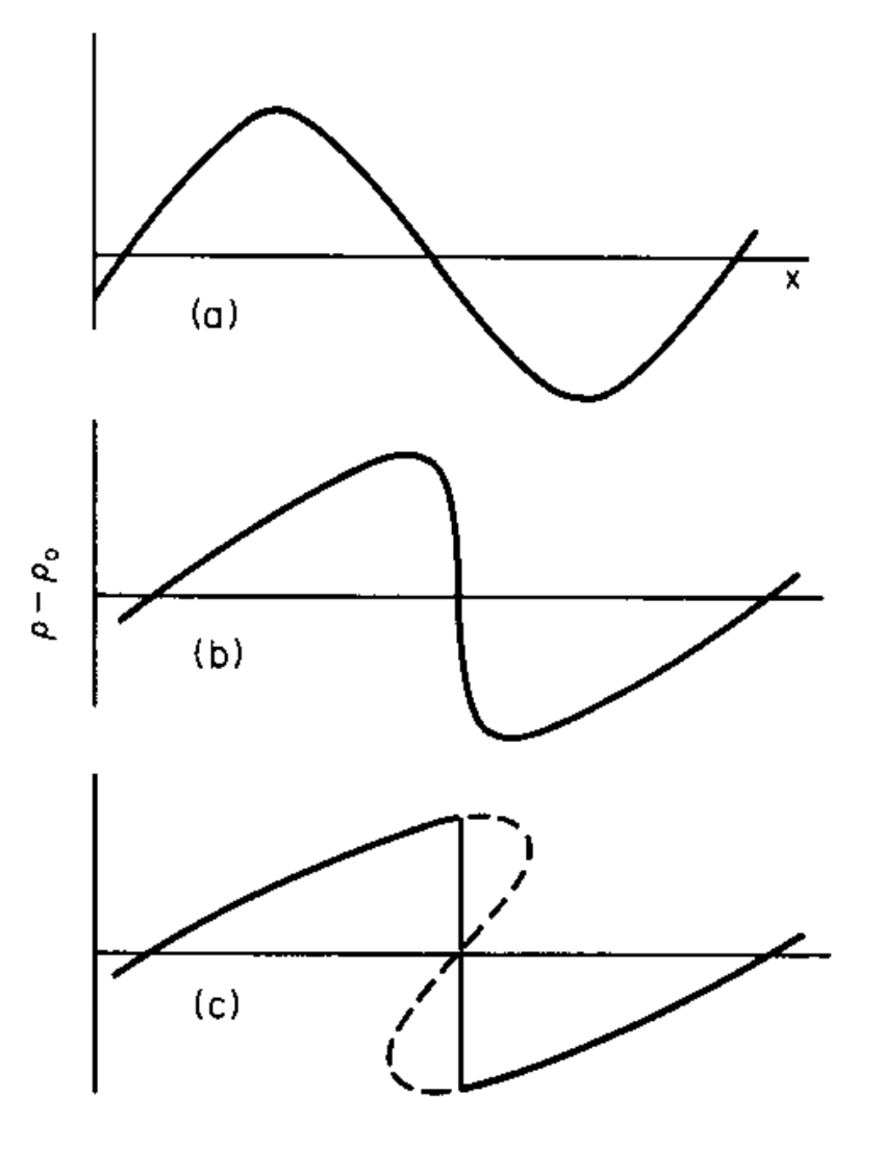
\includegraphics[width=0.5\textwidth]{figures/shocklandau.pdf}
\caption{}
\end{figure}

This section aims to qualitatively illustrate how the formation of shock waves is a natural and, consequently, a frequent phenomenon in various astrophysical environments.

In our previous discussion, we examined the propagation of small perturbations in a medium and determined that they travel at a sound speed denoted by \( c_{s,0} = \sqrt{ \frac{\gamma P_0}{\rho_0}} \). This speed was assumed to be constant (at least in the linear regime) throughout the medium.

However, when we consider sound waves of finite amplitude, we enter the non-linear regime. In this regime, the propagation velocity of the waves is no longer constant but depends on the local density of the medium: the higher the density, the greater the sound speed at that point.


To be checked: \[ c_s = \frac{2 c_{s,0}}{\gamma - 1} \left[ \left( \frac{\rho}{\rho_0} \right)^{(\gamma-1)/2} -1 \right] \simeq c_{s,0} \left( \frac{\delta \rho}{\rho} \right) \]

Consider a waveform as the solution found beforehand. Since this crest represents a region of higher density, it propagates faster than the leading or trailing edges of the wave. Consequently, the crest of the wave, moving fastest, gradually overtakes the trough following it. This overtaking would result in a multi-valued wave profile, which is physically implausible. To resolve this inconsistency, the wave \emph{breaks}, forming a discontinuity known as a shock wave.

%Ultimately, the gradients of pressure, density, temperature and velocity becomes so large that dissipative processes (viscosity) are no longer negligible
%Then a steady wave-shape is attained, called a shock wave, with a balance between the steepening effect of nonlinear convective terms and broadening effect of dissipation.


From this phenomenon, we can glean some insights into the nature of shock waves:
%
\begin{itemize}
\item Shock waves are typically associated with matter moving at a speed \emph{exceeding} the sound speed.
\item The transition to shock wave conditions occurs more rapidly than the medium can adjust or respond to the change.
\item As the shock wave's speed exceeds any signal-bearing speed in the medium, the pre-shock region remains unaware of the impending disturbance. Thus, the alterations in fluid properties (such as density, temperature, and velocity) occur so abruptly that they manifest as discontinuities in these fluid variables.
\end{itemize}


%%% END CGPT

%Slightly non-linear sound waves will steepen to form a discontinuity. formation of a discontinuity.
%In most cases a shock involves a “discontinuous” change of fluid properties over a scale ∼ λ.
%Example of supernova remnant shocks PLOTS.
%The speed of propagation is higher at higher temperature, so the crest of the wave gradually overtakes the trough (T ∝ ργ−1).

%What are places where astrophysical shocks occur?
%
%Cloud-cloud collisions
%HII regions expanding into neutral medium
%Stellar wind encountering medium
%Supernova or GRB blast wave (internal and external shocks) Accretion onto compact objects: spherical or disk
%Accretion onto hydrostatic intracluster medium

\section{Interstellar Shock Waves}

\begin{figure}[!t]
\centering
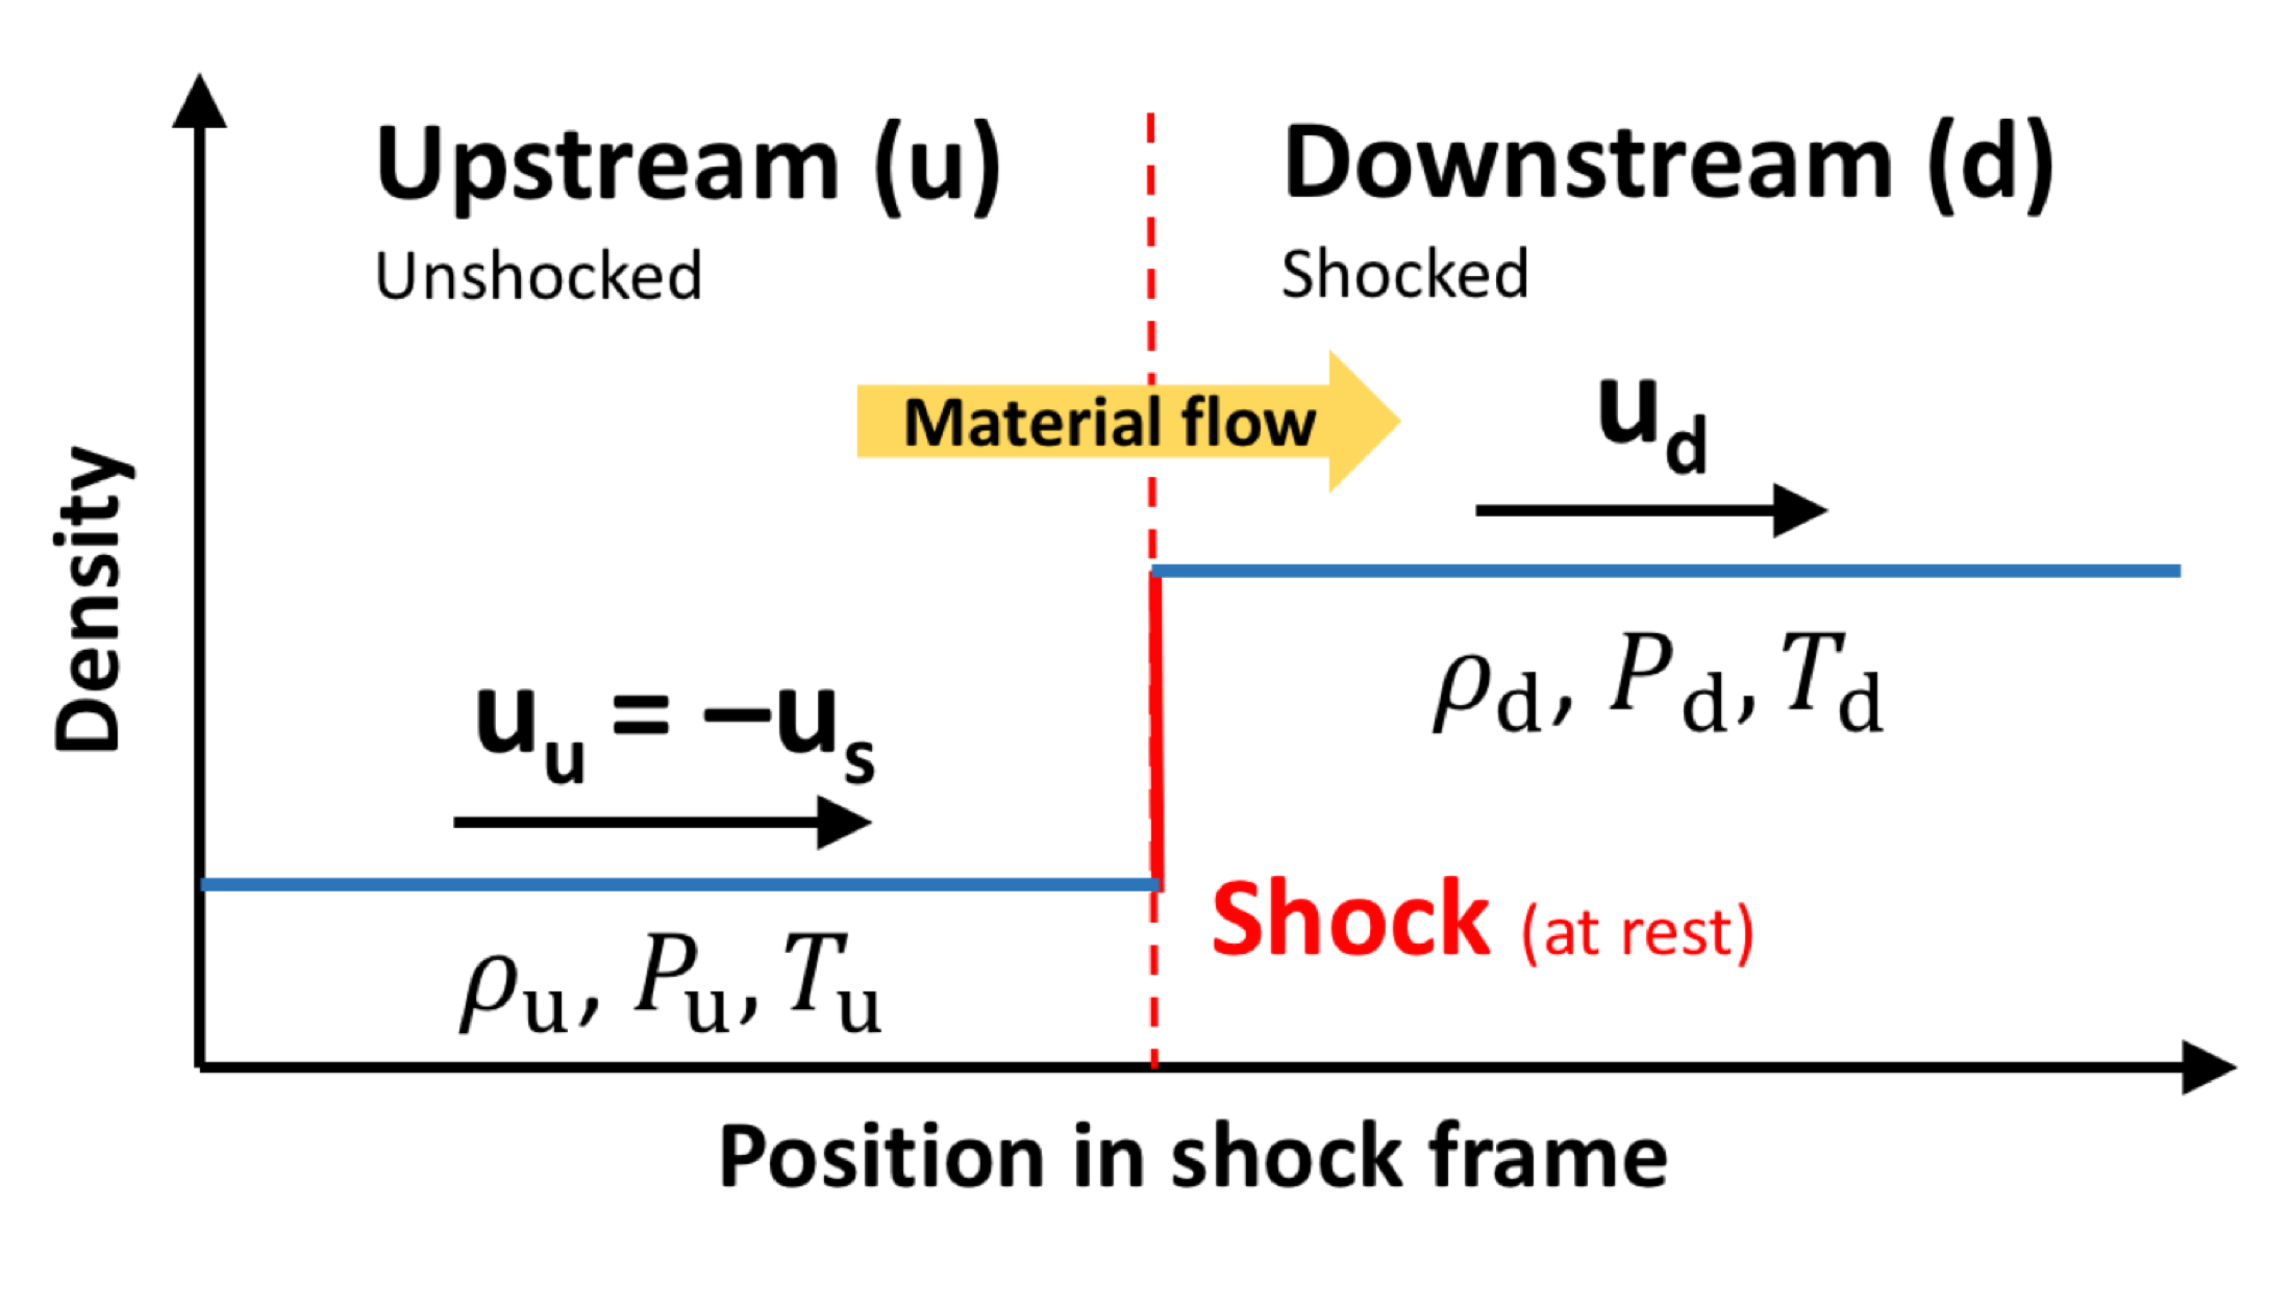
\includegraphics[width=0.5\textwidth]{figures/downupstream.pdf}
\caption{}
\end{figure}

%%% CGPT
Hydrodynamics often presents discontinuous solutions, meaning that there exist surfaces where physical quantities change abruptly. Mathematically, this is represented by differing values at the left and right limits of a point. However, physically, this discontinuity is not infinitely sharp as suggested in mathematical theory; rather, the change occurs over a region smaller than all other physical scales involved. 
%
A \emph{shock} is a specific type of discontinuity characterized by a surface that separates two fluid regions with differing properties. Importantly, this surface allows for the transfer of mass, momentum, and energy across it.

As seen beforehand, shocks are a natural consequence in the non-linear regime of fluid dynamics or magnetohydrodynamics (MHD).

%When the fluid perturbation is so small that linear theory applies, a
%disturbance propagates as a sound wave.{\color{red}Put in appendix sound waves a la Kachelriess?} The wave profile maintains a fixed shape, since each part of wave moves with the same speed.
%But when a disturbance within a fluid grows significantly, the non-linear terms become dominant. This leads to the wave's crest moving faster than its edges, resulting in a steeper wavefront and, eventually, the formation of a shock. 
%
%As a consequence, the shock wave moves at a speed in excess of the sound speed, so information cannot be propagated ahead to signal its imminent arrival.

Shocks are especially relevant in astrophysics; the gas post-shock emits significantly more than pre-shock gas, making these events more detectable.

Unlike terrestrial shocks, astrophysical shock waves are predominantly \textbf{collisionless}. 
%
In standard atmospheric conditions, where the number density of particles is approximately \( n \sim 10^{23} \, \text{cm}^{-3} \), and the cross-section for collisions\footnote{In the case of neutral particles, the hard sphere approximation holds true, where \( \sigma = \pi (r_A + r_B)^2 \) with \( r \) denoting the atomic radii of the colliding atoms.} around \( \sigma \sim 10^{-16}~\text{cm}^2 \), the mean free path \( \lambda \simeq 1 / (n \sigma) \) of a particle is \( \simeq 10^{-7}~\text{cm} \). 
%
In such conditions, \textbf{collisions} between particles are frequent, leading to the transformation of ordered kinetic energy into disordered (thermal) kinetic energy, characteristic of a collisional shock.

In contrast, astrophysical environments, where most particles are ionized, present a different scenario. The cross-sections for ionized particles are typically on the order of \( \sigma \sim \pi r_0^2 \sim 10^{-26}~\text{cm}^2 \) as $r_0 \sim$~fm is now the \textbf{nuclear} radius.
%
More importantly, these environments have much lower particle densities, about \( n \sim 1~\text{cm}^{-3} \). As a result, the mean free path in such settings is \( \gg \) Mpc! 
%
This means that the formation of the shock and its energy dissipation mechanisms do not primarily occur through particle collisions or Coulomb interactions. Instead, these processes are predominantly governed by interactions with the ambient magnetic field. The detailed microphysics of astrophysical shocks are complex and beyond the scope of this discussion.

Despite the microscale complexity at discontinuities (e.g., finite conductivity determining the size), conservation laws of mass, momentum, and energy remain applicable.

For non-relativistic shock waves, we can define the reference frame of the unshocked medium or \textbf{Galaxy frame}, where \( u^\prime_1 = 0 \),
the shock propagates into the unshocked medium at a speed \( u^\prime_s \), while the speed of shocked gas is \( u^\prime_2 (< u^\prime_s) \).

More convenient is to use a frame of reference  where the discontinuity surface is stationary, with \( u_s = 0 \). So the upstream medium approaches it at a speed \( u_1 = -u^\prime_s \), while the shocked fluid moves away from the shock front at a speed \( u_2 = u^\prime_s - u^\prime_2 \).
%
Consequently, the relative speed between the shocked and unshocked fluids is \( u_{\text{rel}} = u_1 - u_2 \).

In the following, it will be easier to refer our equations to the \textbf{shock front frame}, and we will categorize the physical quantities based on their position relative to the shock: those \textbf{upstream} of the shock are labeled as '1' and those \textbf{downstream} as '2'.\footnote{Use instead u and d.}

In the context of shock dynamics, we will focus on key thermodynamic quantities: density, pressure, temperature, and momentum across the two media (upstream and downstream of the shock). To analyze these, we first want to write conservation equations in the form \( \frac{dJ}{dz} = 0 \), where \( J \) represents the flux of a conserved quantity (be it mass, energy, or momentum).

Following this approach, it implies:
%
\begin{equation}
\int_{-\epsilon}^{\epsilon} \frac{dJ}{dx} = J_2 - J_1 = 0
\end{equation}

As common here, we introduce the notation \( [J]_{\text{sh}} = 0\) to denote the change in the flux across the shock expressed as \( J_2 - J_1 = 0 \). 

Let us summarize the key transport equations for a fluid, assuming that the only acting force density is the pressure gradient \( \nabla P \), and neglecting the effects of magnetic or gravitational fields.

First, the mass continuity equation is given by:
%
\begin{equation}
\frac{\partial \rho}{\partial t} + \nabla \cdot (\rho \mathbf{u}) = 0
\end{equation}
%
where \( \rho \) represents the fluid density, and \( \mathbf{u} \) is the fluid velocity.

Next, the conservation of momentum per unit volume is described by:
%
\begin{equation}
\rho \frac{\partial \mathbf{u}}{\partial t} + \rho (\mathbf{u} \cdot \nabla) \mathbf{u} = -\nabla P
\end{equation}

Finally, the conservation of energy per unit volume is expressed as:
%
\begin{equation}
\frac{\partial}{\partial t} \left( \frac{1}{2} \rho u^2 + \rho U \right) + \nabla \cdot \left[ \mathbf{u} \left( \frac{1}{2} \rho u^2 + \rho U + P \right) \right] = 0
\end{equation}
%
here \( \epsilon = \rho U \) denotes the internal energy per unit volume.

For our analysis, we focus on a one-dimensional (planar) shock in a stationary state (\( \partial_t \rightarrow 0 \)) and apply these conservation laws within the reference frame where the discontinuity is stationary.

Applying the mass continuity equation, we derive:
%
\begin{equation}\label{eq:mass}
\frac{\partial}{\partial z} (\rho u) = 0
\end{equation}

Next, from the momentum equation, and utilizing the mass continuity equation in Eq.~\ref{eq:mass}, we obtain:
%
\begin{equation}
\rho u \frac{\partial u}{\partial z} = -\frac{\partial P}{\partial z}  \, \rightarrow \, \frac{\partial}{\partial z} (P + \rho u^2) = 0 
\end{equation}

%Here, \( P_{\text{g}} \) represents the gas pressure.

Moving to the energy equation and again invoking the continuity equation, we find:
%
\begin{equation}
\frac{\partial}{\partial z} \left( \rho u \left[ \frac{1}{2} u^2 + U + \frac{P}{\rho} \right] \right) = 0 
\end{equation}

This can be expressed in terms of specific enthalpy \( w \) (see Appendix):
%
\begin{equation}
w = U + \frac{P}{\rho} = \frac{\gamma}{\gamma - 1}\frac{P}{\rho}
\end{equation}

Therefore, we arrive at the equation:
%
\begin{equation}
\frac{\partial}{\partial z} \left( \frac{1}{2} u^2 + \frac{\gamma}{\gamma - 1}\frac{P}{\rho} \right) = 0 
\end{equation}

Summarizing, assuming planar geometry, and in the frame of the shock, the conservation of fluxes of mass, momentum energy across the shock write
%
\begin{remark}
\begin{eqnarray}
\left[ \rho u \right]_{\rm sh} & = & 0 \label{eq:RH1} \\
\left[ \rho u^2 + P \right]_{\rm sh} & = & 0 \label{eq:RH2} \\
\left[ \frac{1}{2} u^2 +\frac{\gamma}{\gamma - 1} \frac{P}{\rho} \right]_{\rm sh} & = & 0 \label{eq:RH3}
\end{eqnarray}
\end{remark}

These conditions are known as the \textbf{Rankine-Hugoniot jump conditions}. They represent the dynamical equations for solutions that express conservation across the discontinuity of a shock, essentially establishing relationships between quantities on either side of the shock front.

We are dealing with three unknowns and have three corresponding equations. Apart from the trivial solution where all quantities remain constant, our aim is to derive the non-trivial solution.

To proceed, we remind the definition of sound speed:
%
\begin{equation}
c_{\text{s}} = \left( \frac{\partial P}{\partial \rho} \right)^{1/2} = \left(\frac{\gamma P}{\rho}\right)^{1/2}
\end{equation}

Here, we assume an ideal gas so the equation of state is \( P = K \rho^\gamma \), with \( \gamma \) being the ratio of specific heats. For a mono-atomic gas, in particular, \( \gamma = 5/3 \).

We then define the Mach number as the ratio of the shock speed to the sound speed in region \( i \), denoted as \( \mathcal{M}_i = v_i / c_{\text{s}} \). From this, it follows that:
%
\begin{equation}
\rho_i u_i^2 + P_i = \rho_i c_{\text{s}, i}^2 \left( \frac{u_i^2}{c_{\text{s},i}^2} \right) + P_i = (1 + \gamma \mathcal{M}_i^2) P_i
\end{equation}

If we fix the quantities in the upstream region,  $\rho_1$,  $u_1$ and $P_1$, hence solving the equations for the downstream using Eq.s~\ref{eq:RH1}-\ref{eq:RH3} will lead us to (see Appendix):
%
\begin{eqnarray}
\frac{\rho_2}{\rho_1} & = & \frac{u_1}{u_2}=\frac{(\gamma +1) \mathcal M_1^2}{(\gamma - 1) \mathcal M_1^2+2} \\
\frac{P_2}{P_1} & = & \frac{2\gamma \mathcal M_1^2}{\gamma +1}-\frac{\gamma -1}{\gamma +1} \\
\frac{T_2}{T_1} & = & \frac{\left[2\gamma \mathcal M_1^2 -(\gamma - 1) \right] \left[ (\gamma - 1) \mathcal M_1^2 + 2 \right]}{(\gamma + 1)^2 \mathcal M_1^2}
\end{eqnarray}

Under the assumption of strong shock conditions, characterized by \( \mathcal{M}_1 \gg 1 \), and considering a monoatomic gas with \( \gamma = 5/3 \), we can deduce the jump in density:
%
\begin{remark}
\begin{equation}
r = \frac{\rho_2}{\rho_1} = \frac{u_1}{u_2} = \frac{\gamma + 1}{\gamma - 1} = 4
\end{equation}
\end{remark}
%
here, \( r \) represents the compression factor, defined as \( \frac{\rho_2}{\rho_1} \). This factor is dependent on the adiabatic index \( \gamma \) and the Mach number of the shock. It's noteworthy that the compression factor cannot exceed 4.

For the pressure jump, we obtain:
%
\begin{equation}
\frac{P_2}{P_1} = \frac{2 \gamma}{\gamma + 1} \mathcal{M}_1^2 = \frac{5}{4} \mathcal{M}_1^2 
\end{equation}

From the frame of reference at the discontinuity, we observe an approaching gas with velocity \( u_1 \), which is altered to \( u_2 \approx \frac{1}{4}u_1 \) on the opposite side. Consequently, the plasma is decelerated and becomes denser.
%
However, energy conservation dictates that this energy must transform into \textbf{heat}. Examining the temperature ratio \( \frac{T_2}{T_1} \) under the same conditions, we find:
%
\begin{equation}
\frac{T_2}{T_1} = \frac{2 \gamma (\gamma - 1)}{(\gamma +1)^2} \mathcal{M}_1^2
\end{equation}

Therefore:
%
\begin{remark}
\begin{equation}
k_B T_2 = k_B T_1 \frac{2 \gamma (\gamma - 1)}{(\gamma +1)^2} \frac{u_1^2}{c_{\text{s},1}^2} = \frac{3}{16} m_p u_1^2
\end{equation}
\end{remark}

In this equation, we have utilized \( \rho_i = n_i m_p \), \( \mathcal{M}_i^2 = \frac{u_i^2}{c_{\text{s},i}^2} \), \( c_{\text{s},i}^2 = \frac{\gamma P_i}{\rho_i} \), and \( P_i = n_i k_B T_i \).

It's interesting to note that for typical astrophysical shocks, with \( u_1 \gtrsim 10^4 \) km/s, the temperature \( T_2 \) reaches approximately \( \sim 10^7 \) K.
%
This is what happens for example in a supernova explosion \( \mathcal M \sim 10^3 \) or in a GRB.  The plasma crosses shocks and heats up until it starts radiating in X-ray.

In summary, shocks convert \textbf{bulk kinetic energy of upstream medium to thermal (internal) energy downstream}.

\begin{remark}
The plasma behind the shock is
\begin{itemize}
\item Compressed \( \rho_2 = 4 \rho_1 \)
\item Slown down \( v_2 = \frac{1}{4} v_1 \)
\item Heated \( T_2 \ll T_1 \)
\end{itemize}
\end{remark}
%%% CGPT

The transformation of inflow kinetic energy into thermal energy in shock waves is accompanied by the generation of entropy. The key to this transformation is the collisions among particles within the shock wave. These collisions convert the ordered bulk kinetic energy, where particle velocities are aligned, into disordered internal kinetic energy, or heat.

However, as we have previously noted, the mean free path for collisions in astrophysical conditions can be macroscopically large. In such scenarios, energy exchange among particles is mediated by electromagnetic fields.
%
Therefore, the thickness of the shock is more characterized by the non-relativistic Larmor radius of a proton. This radius reflects the scale over which particles are deflected by the magnetic field present at the shock front.

Considering a typical proton velocity of \( \sim 10^4 \) km/s in a supernova explosion, and within a typical galactic magnetic field of \( 1 \mu \)G, the Larmor radius (\( r_{\text{B}} \)) is calculated as:
%
\begin{equation}
r_{\text{B}} = \frac{m_p v c}{e B} \simeq 10^{10}~\text{cm}
\end{equation}

When compared to typical lengths involved in supernova (SN) explosions, which are on the order of a parsec (see later), the shock thickness is several orders of magnitude smaller. Therefore, in the grand scale of such astrophysical phenomena, the approximation of an infinitely thin shock layer is justified.

Finally, we want to compute the post-shock Mach number \( M_2 \):
%
\begin{equation}
\mathcal M_2 = \frac{u_2}{c_{\rm s,2}} = \mathcal M_1 \frac{u_2}{u_1} \frac{c_1}{c_2} = \mathcal M_1 \frac{u_2}{u_1} \left( \frac{T_1}{T_2} \right)^{1/2}
\end{equation}
%
in the strong shock limit:
%
\begin{equation}
\mathcal M_2 = \mathcal M_1 \frac{\gamma - 1}{\gamma + 1} \left[ \frac{(\gamma + 1)^2}{2\gamma(\gamma - 1) \mathcal M_1^2} \right]^{1/2} = \left( \frac{\gamma - 1}{2\gamma} \right)^{1/2} \simeq 0.45 
\end{equation}
%
so a shock converts supersonic gas into subsonic gas.
%
In doing so, it increases the specific entropy of the gas by an amount~(see appendix):
%
\begin{equation}
s_2 - s_1 = c_{\rm P} \ln \left(\frac{T_2}{T_1}\right) - \frac{k}{m} \ln \left( \frac{P_2}{P_1} \right)
\end{equation}
%
In another terminology, a shock changes the entropy shifting gas to a higher adiabat.

Notice then that the non trivial solution makes sense only if the Mach number $M_1$ is larger than one. In the opposite case, we the variation of entropy would be in the sense to decrease it, which is not allowed by second principle of thermodynamics. 
%
In other words we would have invented a system to transform heat in ordered work! Shocks can only form in supersonic motion.

%Rankine-Hugoniot conditions give macroscopic description of shock.

%Energy exchange through electromagnetic interactions (wave-particle inter- actions/reflection). Typical shock scale is thermal particle Larmor radius (a few 100 to 1000 km).

%Particles carrying more energy (injection problem) have larger Larmor radius, and see shock as discontinuity.


\subsection{Supernovae in the Milky Way}

Historical SNe: Kepler 1604, {\color{red}Tycho SNR 1572}, SN1006 SNR, Cas A 1680?

We distinguish between: 
%
\begin{itemize}
\item Core collapse supernovae (Type II, Ib/c,..)
\begin{itemize}
\item Progenitor: Massive star (\( \gtrsim 8~M_\odot \))
\item Energy source: gravitational collapse (\( \gtrsim 10^{53} \)~erg) 
\item Kinetic energy: \( \sim 10^{51} \)~erg
\item Ejecta mass \( >4~M_\odot \)  
\item Neutron star (or BH)
\end{itemize}
\item Thermonuclear supernovae (Type Ia)
\begin{itemize}
\item Progenitor: accreting CO white dwarf, or merging white dwarfs 
\item Energy source: nuclear fusion (C/O -> Fe-group)
\item Kinetic energy: \( 1.2 \times 10^{51} \) erg
\item Ejecta mass \( \sim 1.4~M_\odot \)
\item Total disruption of star
\end{itemize}
\end{itemize}

%Supernova are last phase of the evolution of some stars->huge increase of the star’s luminosity. Show SN 1994D.
%
%Chinese astronomers (and others) reported on the appearance of bright stars. Crab SNR (1059).
%
%All ALL recorded SNe associated with SNRs in the MW
%
%extragalactic SNe + studies of galactic stellar population -> ~3 SN/century in the MW
%
%~1/200 yr -> obscured by interstellar dust
%
%. VVhen these massive stars die, they
%explode as supernovae, releasing about 1051 erg of energy into the
%surrounding medium in ejecta moving at velocities of up to 104 km
%
%About 104 years later, the remnant of a supernova may look like
%the Veil Nebula in Cygnus (part of the Cygnus Loop supernova
%remnant), which is expanding at several hundred kilometers per
%second. Radio and infrared observations have shown that there is
%another type of nebula that is normally obscured from our eyes by
%interstellar dust: high-velocity molecular flows from newly forming
%stars, which have typical injection velocities of order 200 km s- 1.
%The effect of this energy injection depends on the velocity of the
%injected mass relative to the sound speed in the ambient medium.
%
%zoology of SNe.

%{\color{red}Energy budget \( | E_grav = 3/5 GM_c^2/R_c \simeq 10^{53} \)~erg, 99\% into neutrinos's and 1\% into mechanical energy Same source for supernovae (Ib/Ic and II),
%- Explosion powered by the collapse (death) of a massive core
%- Energy source: Potential Energy from the collapse of the iron core down to a neutron star or black hole:Mcore ~ 1.4-3 solar masses
%RNS,BH ~ 10 km
%Rcore ~ 10,000 km} 

\section{Dynamical Evolution of Supernova Remnants}

Our goal is to model the explosion of a SN, which can be approximated as the instantaneous release of energy \( E \) at the origin (\( r = 0 \)) and at the initial moment (\( t = 0 \)). Assuming that the external medium is homogeneous and static, the motion of the resulting shock wave will be symmetrically radial.

In the initial phase of the explosion, the energy released is so immense that the effect of the density \( \rho_0 \) of the surrounding medium is negligible. 
%
This leads to the shock wave propagating at a constant, ballistic velocity, a stage known as the \emph{Free Expansion Phase}.

During this phase, an amount of matter \( M_{\rm ej} \) is ejected with velocity \( v_0 \) and kinetic energy \( E_{\rm SN} \). From this we can derive the constant velocity:
%
\[
E_{\rm SN} = \frac{1}{2} M_{\rm ej} v_0^2 \rightarrow v_0 = 10^4 \left( \frac{E_{\rm SN}}{10^{51}~\text{erg}} \right)^{1/2} \left( \frac{M_{\rm ej}}{M_\odot} \right)^{-1/2}~\text{km/s}
\]

This ejection velocity can be compared with the sound speed \( c_{\rm s} \) in the ISM:
%
\[
c_{\rm s} = \left( \gamma \frac{k T}{m_p} \right)^{1/2} \simeq 10 \left( \frac{T}{10^4~\text{K}} \right)^{1/2}~\text{km/s}
\]

For a monoatomic gas, \( \gamma = 5/3 \). Given these conditions, the Mach number (\( \mathcal M \)) is approximately \( 10^3 \), indicating that a \emph{strong} shock is indeed produced.

The evolution of the supernova remnant during this phase can be described simply by:
%
\begin{eqnarray*}
v_s & =  & v_0 \\
R_s & = & v_0 t 
\end{eqnarray*}

This phase is characterized by the shock wave expanding outward at a constant velocity, unimpeded by the surrounding medium.
 
 %%%
 
% supernova che possiamo considerare come il rilascio improvviso di energia E in un volume trascurabile per r “ 0 e t “ 0. Se il mezzo esterno `e omogeneo e statico (⇢0 “ cost., ~v0 “ 0), il moto dell’onda d’urto che si genera per r “ 0 sar`a radialmente simmetrico. Suppo- nendo poi che il mezzo sia ”freddo” (T0 “ 0, ovvero temperatura trascurabile rispetto al mezzo post-shock), possiamo trovare la forma delle soluzioni con argomenti di auto-similarita` usando soltanto i dati a disposizione, ovvero E e ⇢0. Vogliamo ottenere Rsptq e Vsptq ovvero il raggio dell’onda d’urto e la sua velocita` in funzione del tempo.
%
 
The free expansion phase remains valid under the condition that the mass \( M_{\rm sw} \) swept up by the shock is negligible compared to the mass \( M_{\rm ej} \) of the ejecta:
%
\[
M_{\rm ej} \gg M_{\rm sw} \simeq \frac{4\pi}{3} R_s^3 \rho_0
\]

This condition ensures that the momentum of the ejecta is largely unaffected by the interstellar medium. However, as the shock wave expands, it accumulates more interstellar material, increasing \( M_{\rm sw} \).

Notice that shock waves generated by SN explosions may propagate through the ISM, or through the \emph{wind} of the progenitor star, where the density, \( \rho_0 \) is much smaller, hence the free expansion phase is longer.

When the swept-up mass becomes comparable to the ejecta's mass, the expansion of the remnant inevitably slows down. 
%
This transition occurs at a distance, denoted as \( R_{\rm ej} \), which can be approximated when \( M_{\rm ej} \simeq M_{\rm sw} \):
%
\[
R_{\rm ej} \simeq 2 \left( \frac{M_{\rm ej}}{M_\odot} \right)^{1/3} \left( \frac{n_0}{\text{cm}^{-3}} \right)^{-1/3}~\text{pc}
\]

Correspondingly, a characteristic time \( t_{\rm ej} \) can be determined for this phase:
%
\[
t_{\rm ej} \simeq \frac{R_{\rm ej}}{v_0} \simeq 2 \times 10^2 \left(\frac{M_{\rm ej}}{M_\odot}\right)^{5/6} \left(\frac{E_{\rm SN}}{10^{51}~\text{erg}}\right)^{-1/2} \left(\frac{n_0}{\text{cm}^{-3}}\right)^{-1/3}~\text{year}
\]

As the shock wave expands through the surrounding medium, it sweeps up and accumulates material, pushing it into a thin shell at the shock front. To estimate the thickness of this shell, we compare the total mass accumulated with the mass in a shell where the density is \( 4 \rho_0 \), reflecting the compression of the downstream material:
%
\[ \frac{4\pi}{3} R_{\rm s}^3 \rho_0 = 4 \pi R_{\rm s}^2 \Delta R (4 \rho_0) \]

From this, we derive the relative shell thickness: \[ \frac{\Delta R}{R_{\rm s}} = \frac{1}{12} \sim 10\% \] 

This calculation confirms the validity of the \emph{thin shell approximation}, indicating that the accumulated material forms a relatively narrow layer compared to the overall radius of the shock wave.

We can express the mass within this shell as:
%
\[
M = \cancel{M_{\rm ej}} + 4\pi \int_0^{R_{\rm s}} dR R^2 \rho_0 \simeq \frac{4\pi}{3} R^3_{\rm s} \rho_0
\]
%
where we assume that the mass of the ejecta is negligible compared to the mass of the swept-up material.

The expansion of the shock wave occurs adiabatically. In fact, for temperatures \( T \gtrsim 10^6 \)~K, the radiative cooling of the post-shocked gas is extremely inefficient as the cooling timescale is significantly longer than the expansion timescale of the shock wave. 

Given this adiabatic condition, we can apply the {\color{red}energy conservation equation}:
%
\[
E = E_k + E_{\rm th} 
= \frac{1}{2} M v_{\rm sh}^2 + \epsilon \frac{4\pi}{3} R^3_{\rm s} 
= \frac{1}{2} M v_{\rm sh}^2 + \frac{P_{\rm in}}{\gamma - 1} \frac{4\pi}{3} R^3_{\rm s} 
= \text{const}
\]

In the Sedov phase of SNR expansion, momentum conservation is governed by the equation:
%
\[
\frac{d}{dt} \left(M v_{\rm sh} \right) = 4\pi R^2_{\rm s} (P_{\rm in} - \cancel{P_{\rm out}})
\]

In the case of a strong shock, the external pressure \( P_{\rm out} \) is negligible compared to the over-pressurized internal gas, and thus it is omitted from the equation.

Seeking power law solutions, we propose a form for the shock radius:
%
\[ 
R_{\rm s} = A t^\alpha \rightarrow v_{\rm s} = \frac{dR_{\rm s}}{dt} = \frac{\alpha R_{\rm s}}{t} \propto t^{\alpha - 1}
\]

With this form, the momentum equation transforms into (using \(\gamma = \frac{5}{3} \)):
%
\[
\frac{\rho_0}{4} \frac{d}{dt} (R_s^3 v_s) = R_s^2 P_{\rm in} \rightarrow P_{\rm in} = \frac{(4\alpha - 1)}{4\alpha} \rho_0 v_s^2
\]

Here, we utilize the mass expression from a previous equation and the velocity relation downstream, \( v_{\rm sh} = \frac{3}{4} v_s \).

Consequently, the total energy of the system is given by:
%
\[
E = \frac{\pi}{8} \rho_0 A^5 \alpha (19 \alpha - 4) t^{5\alpha-2}
\]

Since the Sedov phase is characterized by constant total energy, the value of \( \alpha \) and \( A \) are determined as:
%
\[ 
\alpha = \frac{2}{5} \quad \text{and} \quad A = \left( \frac{50}{9\pi} \frac{E_{\rm SN}}{\rho_0} \right)^{1/5} 
\]

We conclude that during the Sedov phase, the energy distribution is such that one-third of the total energy is kinetic (\( E_k / E = 1/3 \)), while two-thirds is thermal (\( E_{\rm th} / E = 2/3 \)). 

%%% END CGPT

%We know \( M = \frac{4\pi}{3} \rho_0 R^3_s \) , \( \gamma = 5/3 \), \( v_{\rm sh} = 3/4 v_s \)
%{\color{red}shell speed - shock speed}

By substitution we find the evolution equation for radius and velocity
%
\[
R_{\rm s} \simeq 5~\left(\frac{E_{\rm SN}}{10^{51}~\text{erg}}\right)^{1/5} \left(\frac{n_0}{\text{cm}^{-3}}\right)^{-1/5} \left(\frac{t}{\text{kyr}}\right)^{2/5}~\text{pc}
\]
%
and
%
\[
v_{\rm s} \simeq 2 \times 10^3~\left(\frac{E_{\rm SN}}{10^{51}~\text{erg}}\right)^{1/5} \left(\frac{n_0}{\text{cm}^{-3}}\right)^{-1/5} \left(\frac{t}{\text{kyr}}\right)^{-3/5}~\text{km}~\text{s}^{-1}
\]

To determine the end of the Sedov phase we need to compute the cooling timescale, \( \tau_{\rm cool} \), and determine at which age the shell become radiative which corresponds to \( t_{\rm age} \sim \tau_{\rm cool} \)

The cooling time is given by the thermal energy divided the cooling rate
%
\[
\tau_{\rm c} \simeq \frac{\epsilon_{\rm th}}{n_i n_e \Lambda} \simeq \frac{3 \cancel{n} k_{\rm B} T}{n^{\cancel{2}} \Lambda} \simeq 10^6 \left( \frac{n_0}{\text{cm}^{-3}} \right)^{-1} \left( \frac{v_{\rm s}}{10^3~\text{km/s}} \right)^3~\text{yr}
\]
%
where we assumed full ionized gas \( n_i \sim n_e \) and for the cooling function we adopted a value derived from~\cite{}
%
\[
\Lambda \simeq 2 \times 10^{-19} T^{-1/2}~\text{erg}~\text{cm}^3~\text{s}^{-1}
\]

Using the cooling time just derived we find that the shell becomes radiative at an age:
%
\[
t_{\rm S} \simeq 2 \times 10^4 \left( \frac{E_{\rm SN}}{10^{51}~\text{erg}}\right)^{3/14} \left( \frac{n_0}{\text{cm}^{-3}} \right)^{-4/7}~\text{yr}
\]

\[
R_{\rm S} \simeq 20 \left( \frac{E_{\rm SN}}{10^{51}~\text{erg}} \right)^{1/14} \left( \frac{n_0}{\text{cm}^{-3}} \right)^{1/7}~\text{km}~\text{s}^{-1}
\]

%      The energies stay approximately constant over this phase, with only slight adjustment in kinetic and thermal energies once they reach the equilibrium value. The distinction between the shell and the bubble is not rigorous during this phase, since the thin shell has not yet formed. Therefore, the values associated with the shell or the bubble should be taken with caution. It is clear from the plots that the dynamical behavior of the SNR is not influenced until the cooling is near the maximum.

%  Toward the end of the Sedov-Taylor phase, the effect of cooling in the density-enhanced shock front region gradually becomes significant and begins to influence the dynamical evolution. The pressure just behind the shock front decreases due to the temperature drop

% https://iopscience.iop.org/article/10.1086/305704/fulltext/36680.text.html